\documentclass[11pt,reqno]{article}
\usepackage{amsmath,amssymb,mathrsfs,amsthm}
\usepackage[UTF8]{ctex}
%\usepackage{xeCJK}
%\setCJKmainfont{SimSum}

\usepackage{graphicx,cite,cases}
%\usepackage[pagewise]{lineno}\linenumbers
%\usepackage{refcheck}
\usepackage{xcolor}
\usepackage{bm}			% 公式加粗
\usepackage{tabularx}   % 绘制定宽表格
\usepackage{dcolumn}	% 表格横向合并
\usepackage{multirow}	% 表格纵向合并
\usepackage{booktabs}	% 三线表
\usepackage{authblk}	% 添加更多作者信息
\usepackage{appendix} 	% 生成附录
\usepackage{listings}   % 附录里的代码, 支持语言高亮
\usepackage{hyperref}   % 超链接, 自动跳转
\usepackage{subfigure}  % 插入多张图片
\usepackage{tikz}		% 代码作图


\setlength{\topmargin}{-1.5cm}
\setlength{\oddsidemargin}{0.0cm}
\setlength{\evensidemargin}{0.0cm}
\setlength{\textwidth}{16.7cm}
\setlength{\textheight}{23cm}
\headheight 20pt
\headsep    26pt
\footskip 0.4in

%%%%% 关于公式编号问题 %%%%%
%统一用equation环境
%如果需要加括号用\begin{cases}
%如果公式过长需要分行用\begin{split}
%如果一个equation里面需要多个公式, emmm没研究过

\newtheorem{theorem}{Theorem}[section]
\newtheorem{corollary}[theorem]{Corollary}
\newtheorem{lemma}[theorem]{Lemma}
\newtheorem{proposition}[theorem]{Proposition}
\newtheorem{remark}[theorem]{Remark}
\newtheorem{definition}[theorem]{Definition}
\numberwithin{equation}{section}


\renewcommand{\d}{\,\mathrm d}
\usepackage{algorithm,algorithmicx}  %写伪代码
\usepackage{algpseudocode}			% 写伪代码
%%%%%% 算法部分改为中文显示 %%%%%%%%%
%%\floatname{algorithm}{算法}
\renewcommand{\algorithmicrequire}{\textbf{Input:}}
\renewcommand{\algorithmicensure}{\textbf{Output:}}

%% Ctrl+Alt+R 编译
%% Ctrl+Alt+V 打开文档

\begin{document}

\title{微分方程数值解计算实习Lecture 12}

\author{朱荃凡}
\affil{(吉林大学数学系计算唐班)}
\date{\today}

\maketitle

\vspace{50pt}

如图所示,\ $\Omega$表示$[0,1]^2$的区域:
\begin{center}
	\begin{tikzpicture}[scale=2.5]
		% 绘制坐标轴
		\draw[->] (-0.2,0) -- (1.3,0) node[below] {$x$};
		\draw[->] (0,-0.2) -- (0,1.3) node[left] {$t$};
		% 绘制坐标轴标签
		\foreach \x in {}
			\draw (\x,0.05) -- (\x,-0.05) node[below] {$\x$};
		\foreach \y in {}
			\draw (0.05,\y) -- (-0.05,\y) node[left] {$\y$};
		% 绘制矩形
		\draw[fill=gray!20] (0,0) rectangle (1,1);
		\node[below left] at (0,0){$O$};
		\node[below] at (1,0){$(1,0)$};
		\node[left] at (0,1){$(0,1)$};
		\node[right] at (1,1){$(1,1)$};
		\node[above right] at (0.4,0.4){$\Omega$};
	\end{tikzpicture}
\end{center}
分别用求解向前差分,向后差分和六点对称差分进行求解区域$\Omega$上的抛物型方程:
\begin{equation}\label{Eqn1}
	\left\{\begin{matrix}
		\dfrac{\partial u}{\partial t}=\dfrac{\partial^2 u}{\partial x^2}
		+\sin(\pi x)+\pi^2t\sin{\pi x},&\ (x,y)\in\Omega,\\
		u(x,0)=\sin(\pi x),&0\le x\le 1,\\
	   u(0,t)=u(1,t)=0,&0\le t\le 1.,
	   \end{matrix}\right.
\end{equation}
其相应的的真解为
\begin{equation}
	u^*=e^{-\pi^2t}\sin(\pi x)+t\sin(\pi x).
\end{equation}
并给出相应算法在$t=1$时刻的0-范数收敛阶.

\newpage

\section*{程序结果}

在程序中, 我使用了矩阵运算的方式去一次生成一整行的函数值.取$x$轴步长$h=1/16$,网比
$r=16$, 使用向后差分法画出了如下的函数图像:

\begin{figure}[h]
	\centering
		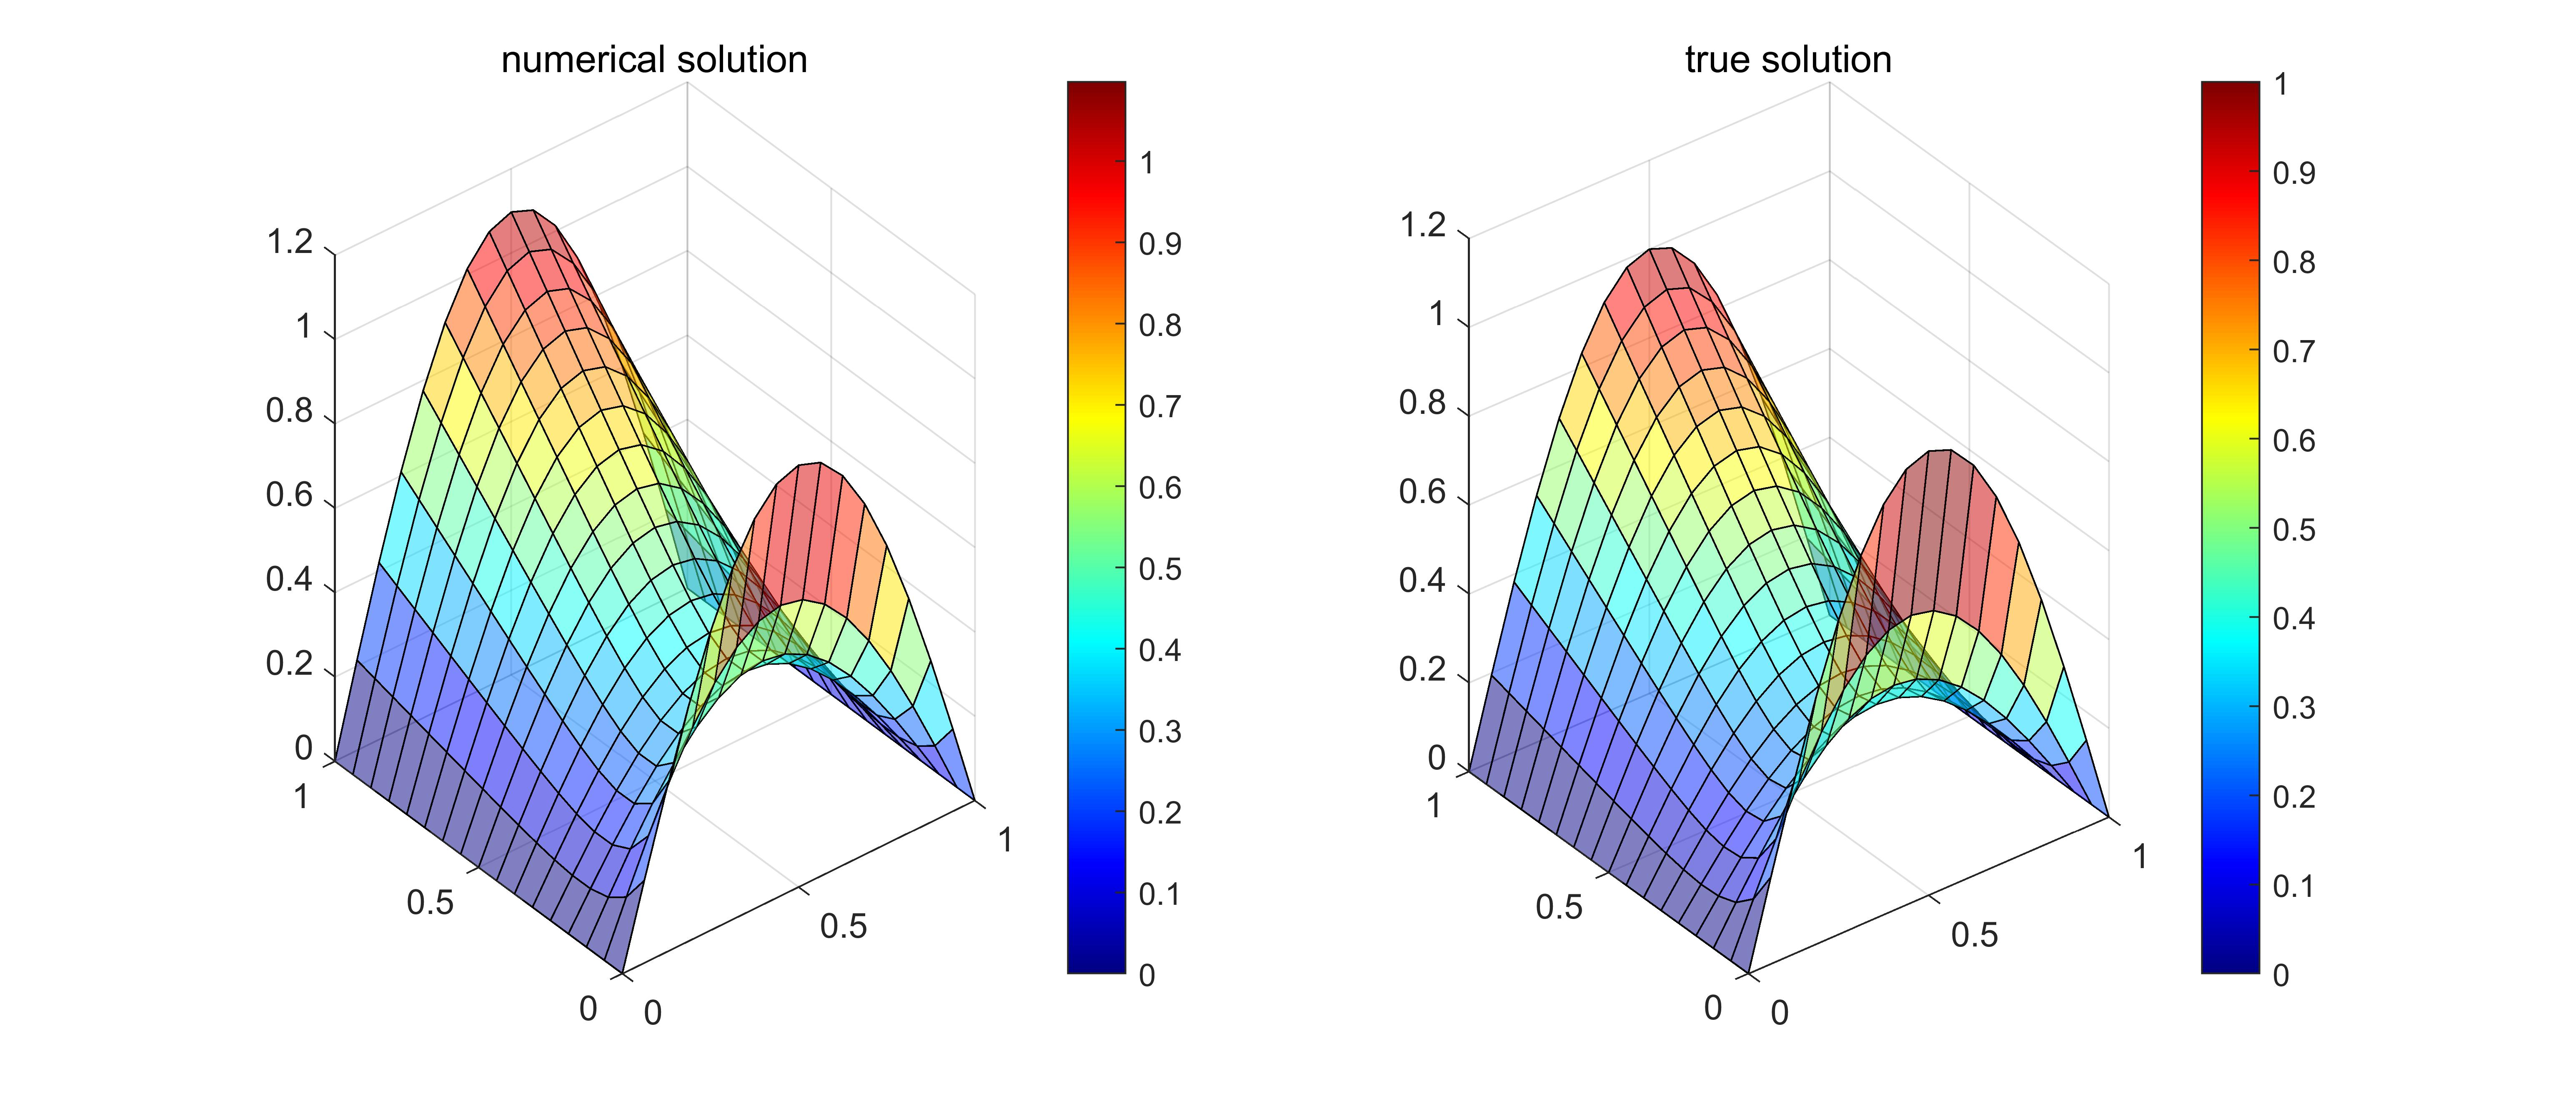
\includegraphics[width=0.9\textwidth]{functionpic.jpg}
\end{figure}


然后在$r=1/2$的情况下, 画出了三种差分格式在$t=1$处的0-范数收敛阶.可以看出三种
格式下的收敛阶均为二阶,并且向后差分格式稍好一些.
\begin{figure}[h]
	\centering
		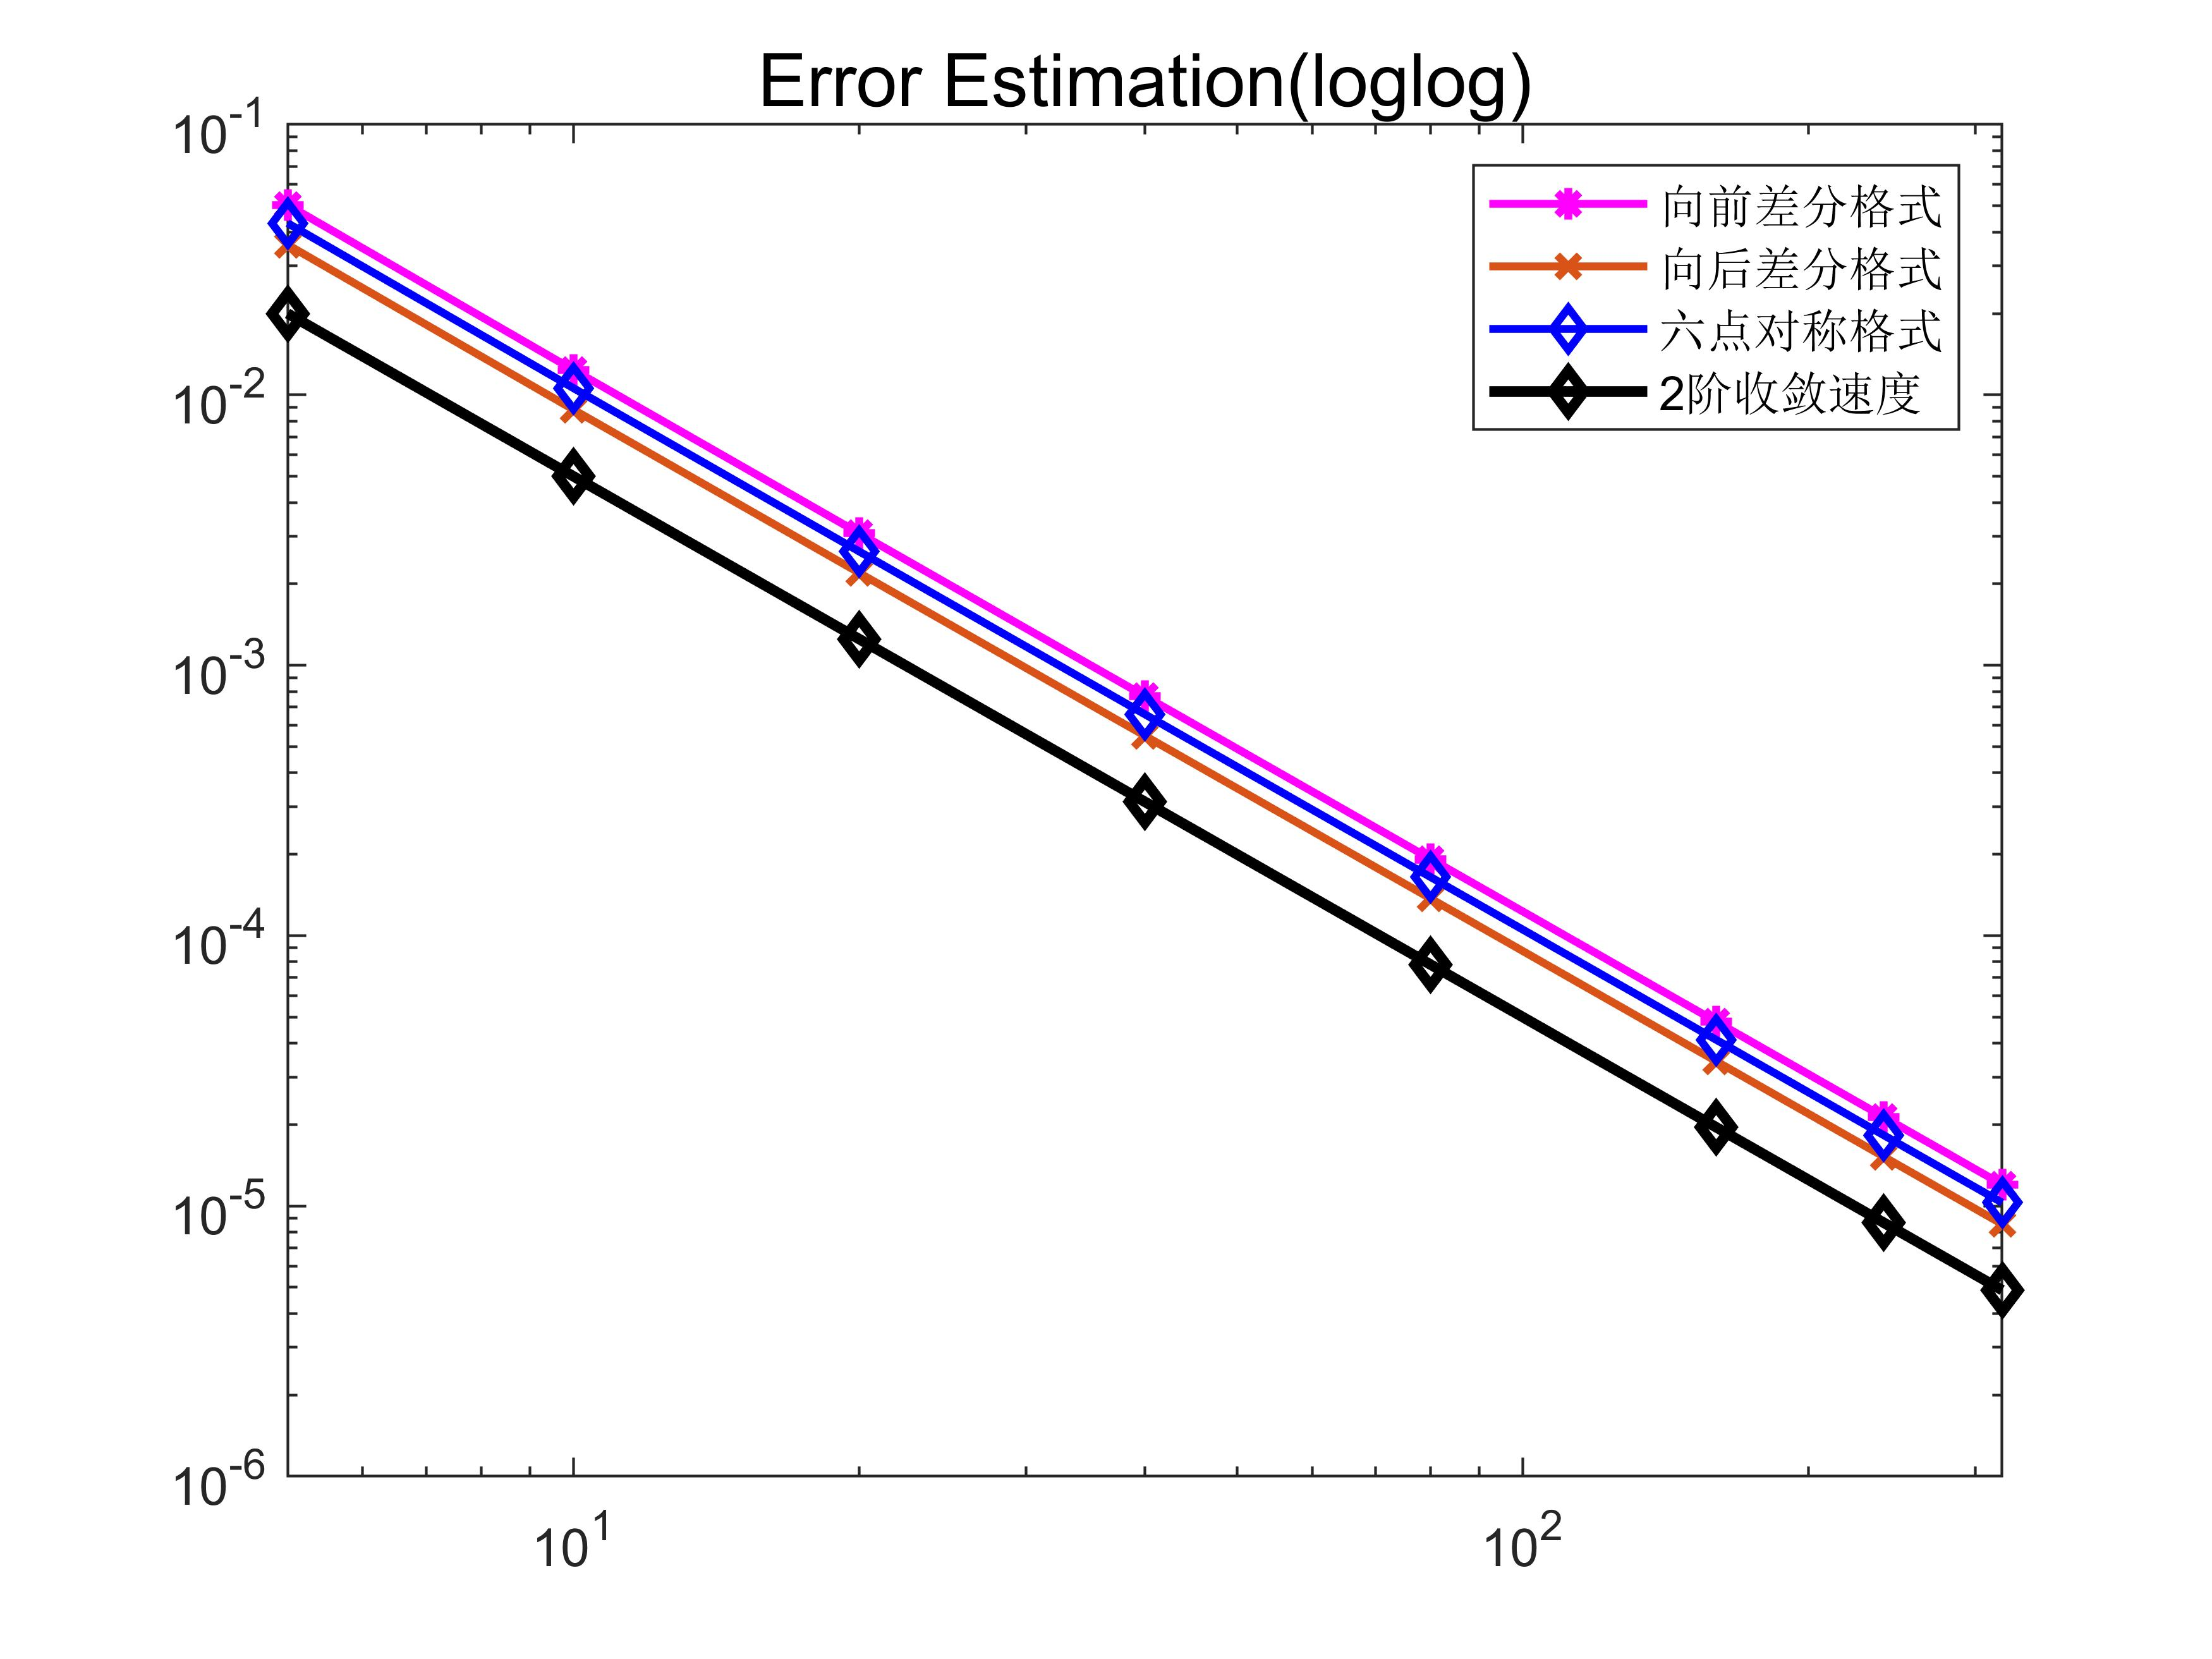
\includegraphics[width=0.6\textwidth]{error.jpg}
\end{figure}



\end{document}
